\chapter{Implementation}
\label{cpt:Implementation}

In this chapter, a practical realization is presented which implements a redundant architecture that applies a consensus algorithm based on the concepts of \texttt{Raft}.
The aim of this implementation is to showcase the practicability and performance of a redundant architecture that applies \abr{DCPS} concepts for finding a consensus in an \abr{ETCS} context, even in the presence of single component failures.
In addition, a minimal required subset of \abr{DDS} features will be carved out to implement the architecture.
This has the potential to safe costs during implementation and system approval.
\\

\begin{figure}[!hb]
	\centering
	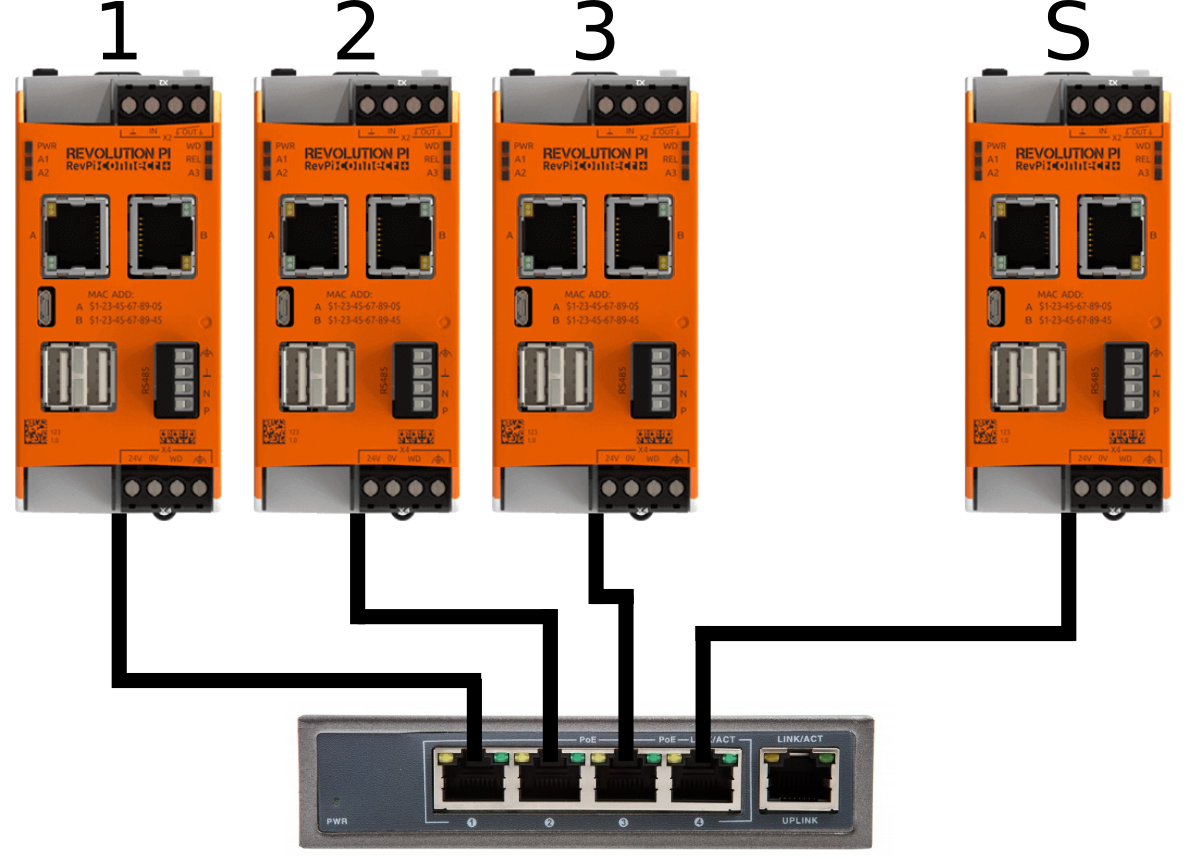
\includegraphics[width=0.7\linewidth]{images/setup}
	\caption{Three \textit{Revolution Pis Connects} make up the redundant system which is implemented in the course of this thesis. The replicas are interconnected via a network switch. A fourth \textit{Revolution Pis Connect} acts as a spare unit and can be activated if needed.}
	\label{fig:SystemSetup}
\end{figure}

The system setup is depicted in~\autoref{fig:SystemSetup}, where four replicas are interconnected via a network switch.
Because of the network switch being a single point of failure in the applied star network, a fully connected network would be the better choice.
A star network does not change the functionality of the setup and was therefore chosen for the demonstration for cost reasons.

While three replicas are operating in a \abr{TMR} setup, the fourth is used as a spare unit that can be patched in on demand, for example when an other replica failed.

Each replica is represented by a \textit{Revolution Pi Connect}, an open source \abr{PLC} that builds upon a Raspberry Pi and is developed by \texttt{Kunbus}.
As such, it features a Broadcom BCM2837 quad core ARM Cortex A53 1.2 GHz \abr{CPU} and 1 GB RAM.
Further, a hardware watchdog is applied that can be configured to react when the program stops responding.
For implementing this, a watchdog timer is deployed that needs to be manually resetted by an application.
When this is not done for a certain period of time, the system assumes that the application crashed and the system is restarted.
A watchdog is an important safety-feature and proposed by Sakic and Kellerer~\cite{SakicTimeInConsensus} to increase a system's probability to response when a component failed.
The used \abr{OS} is an extended \textit{Raspbian} \abr{OS} that has been patched with real-time support.
The solution is implemented in the C programming language and makes use of the C \abr{API} of \textit{Votex OpenSplice DDS} by \texttt{ADLINK}.

The communication channel is implemented via \textit{Ethernet} and no information redundant communication channel is applied in this demonstration.
Further, no N-version programming is applied, which means that each replica runs the same software implementation.
In addition, it is assumed that all replicas function as intended, so that component checking mechanisms are neglected in this implementation.
In order to build a highly secure system, the mentioned compromises need to be further addressed.

\begin{figure}[!hb]
	\centering
	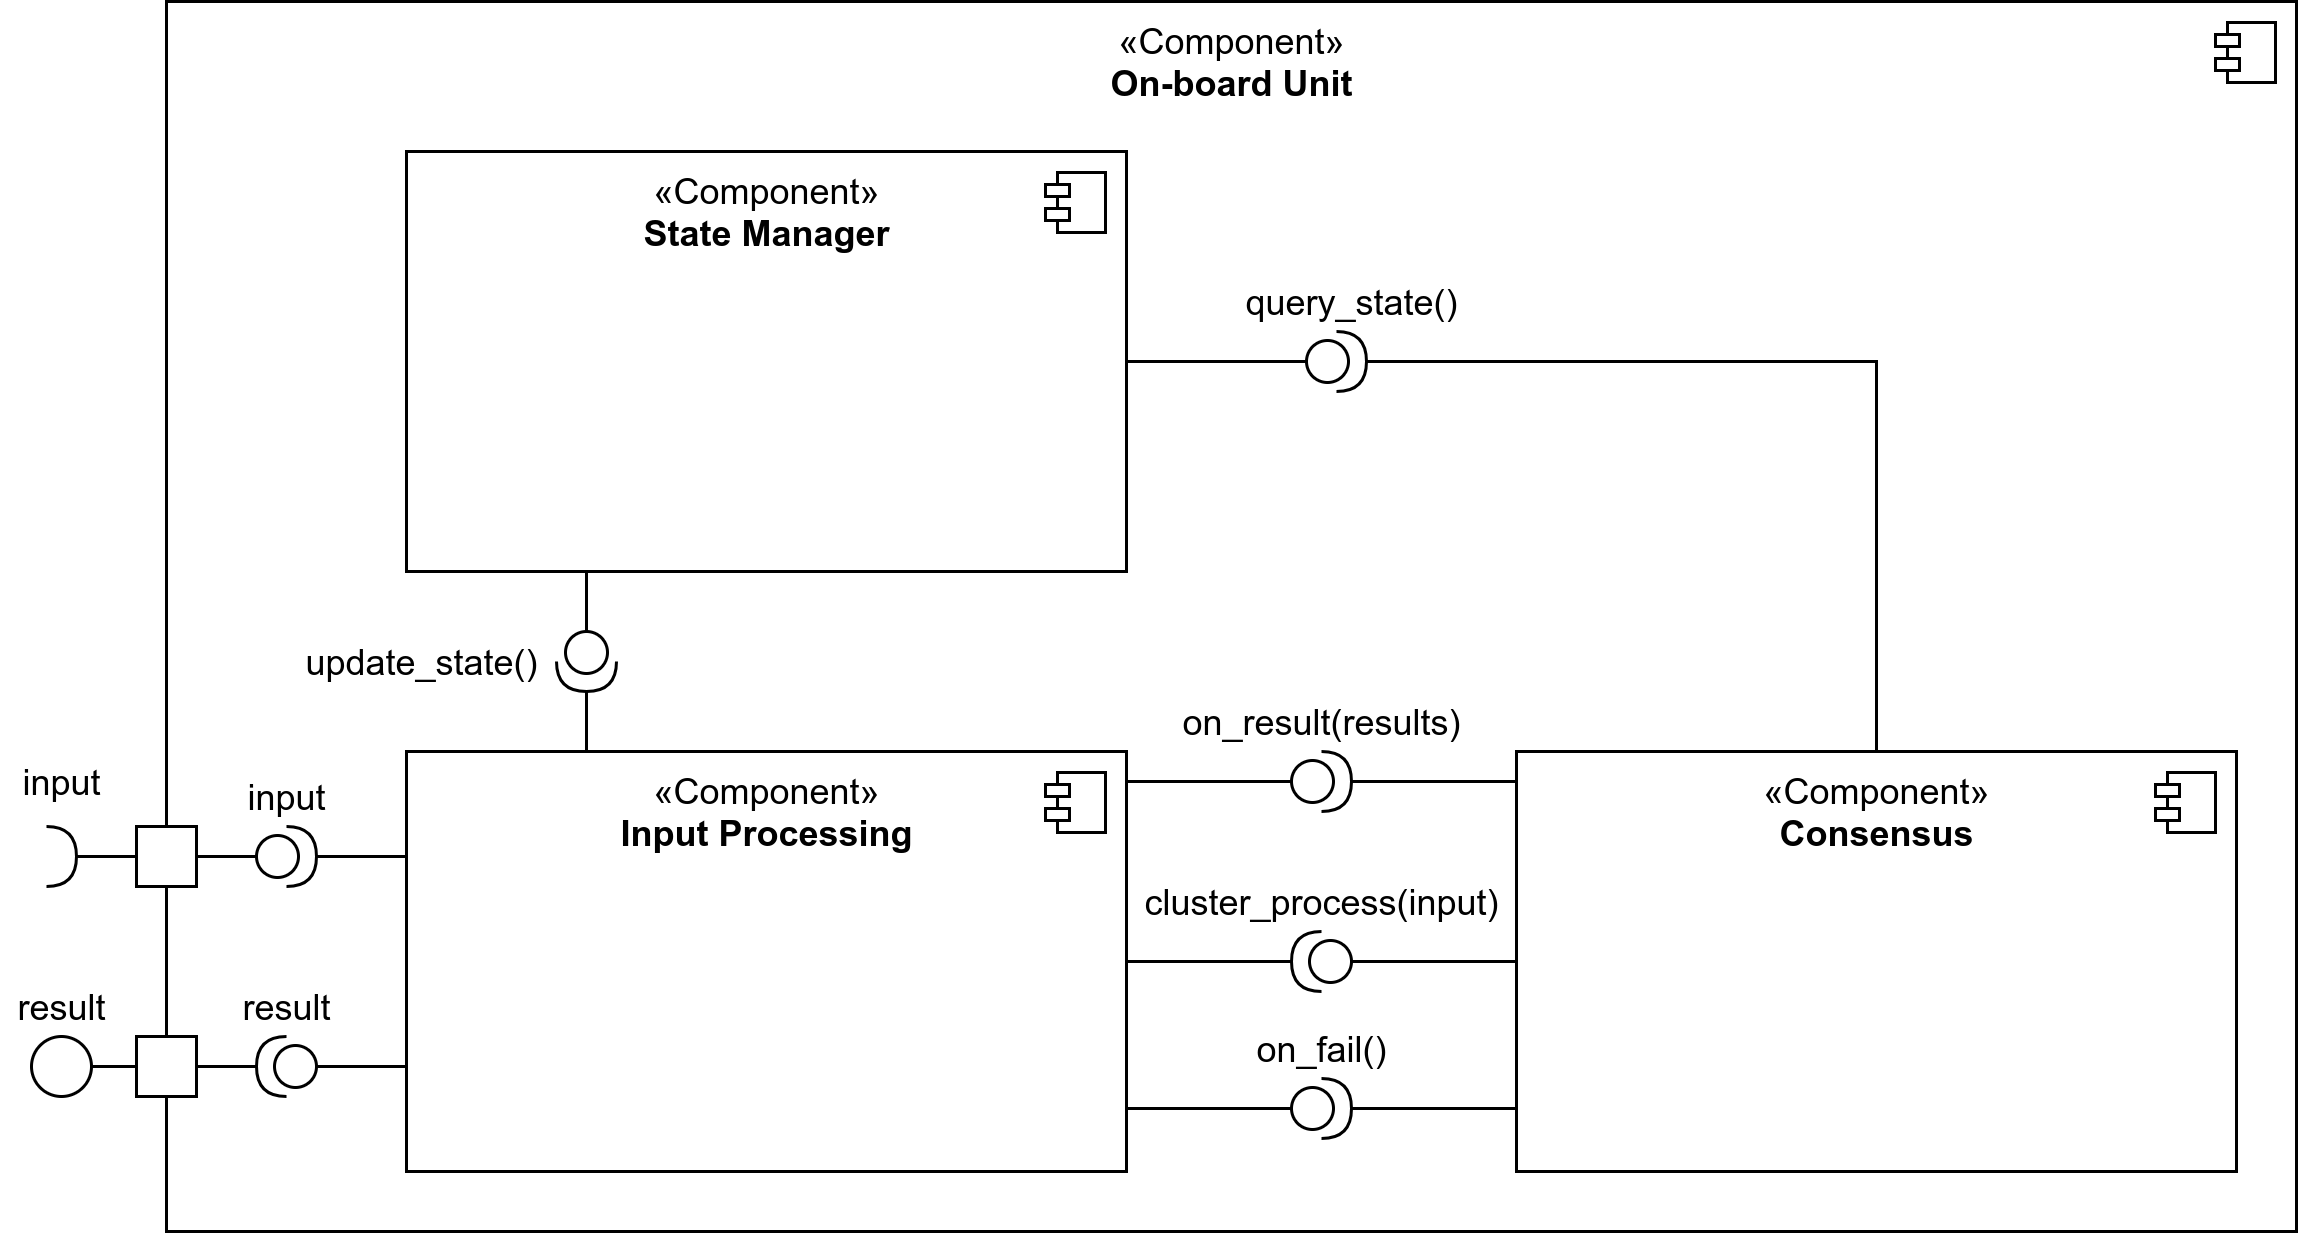
\includegraphics[width=0.9\linewidth]{images/Components}
	\caption{The on-board unit's program, that runs on each replica, consists of three major components. The \texttt{input} processing reads inputs and performs the voting. While the \texttt{state manager} components administers the system's global state, the \texttt{consensus} component ensures that a leader is present in the system and provides an interface to process an input on the cluster and collect all results.}
	\label{fig:SystemComponents}
\end{figure}

A general outline of the system is structure is provided in~\autoref{fig:SystemComponents}.
The system's \texttt{Input Processing} component provides an interface to channel balise or \abr{RBC} telegram messages as inputs and an output where the final result for a corresponding input is presented.
The final result is generated by invoking the \texttt{Consensus} component's \textit{cluster\_process} interface.
Thereby, the input is distributed across the cluster using \abr{DDS} topics and intermediate results are collected.
When enough intermediate results are generated within a certain time-span, \textit{on\_result} is called, otherwise \textit{on\_fail} would be invoked so that the \texttt{Input Processing} component could initiate appropriate consequences.
The \texttt{Consensus} component manages the leader election process, as well as a private replica state.
However, every other decision, that is independent of the consensus algorithm, is made based on a global system state.
This global state is managed by a corresponding \texttt{State Manager} component.

The individual components are described in more detail later in this chapter.
At first in this chapter in~\autoref{sec:ImpScenarioDescription}, a subset of \abr{ETCS} is mapped out that serves as the practical scenario for the implemented system.
Afterwards,~\autoref{sec:ImpConsensusAlgorithm} describes a consensus algorithm, as part of the \texttt{Consensus} component, that builds on \abr{DDS} and ensure that the redundant system can agree on a certain result for each processed input telegram.
Therefore, a leader election process is described, which follows the concepts of \texttt{Raft}, and timing requirements will be taken into account to ensure safety in the redundant system.
The leader election process lays the foundation for the way of how input telegrams are spread across the system and merged into a single final value, which is further described in~\autoref{subsec:ImpBaliseProcessing}.
Thereafter, is is described how the \texttt{State Manager} component manages the system's state and how the state can be updated and queried.
Finally in this chapter, an approach for implementing a simulator is described before a hot standby scenario with \abr{DDS} features is presented.

\section{Scenario Description}
\label{sec:ImpScenarioDescription}
The exemplary implementation, that is described in the following of this chapter, shall comply with \abr{ETCS} level two and receive, evaluate, as well as react to certain \abr{RBC} and track-side balise telegram inputs.
In \abr{ETCS} level two, track-side balises are solely used for detecting and correcting the train's exact position.
As stated in the \abr{ETCS} specification, track-side balises are organized in groups and the combination of all telegrams from balises that belong to a group form a balise group telegram~\cite{ETCS26}.
Each balise group contains at least one and maximal eight balises.
Besides telegrams, each balise group is assigned with a coordinate system that encodes its orientation, and a position.
Therefore, track-side balises can be used both for transmitting information to a on-board unit and for correcting the confidence interval, which means adjusting a trains calculated position.
In order to do so, the expected position of each balise group, which the operating train will encounter on its route, is communicated pre-journey during a linking step.
When a train does not locate a balise group where it is expected, or registers an unlinked balise group, appropriate actions must be taken to ensure safety.

Another important information for a safe train operation is a \abr{MA}, which indicates a location up to which a train is authorized to move, as well as a speed profile and a gradient profile.
In order to ensure compliance with a \abr{MA}, the on-board unit must continuously monitor the train's speed, position, and breaking curve so that it does not disregard the track's profiles or pass the \abr{MA}'s end location.
In \abr{ETCS} level two, \abrpl{MA} with speed and route information are continuously transmitted to the train via wireless communication technologies, such as \abr{GSMR}, from the \abr{RBC}.

It is the on-board unit's responsibility to supervise the train's position, speed, movement authorities and braking curve, as well as to evaluate balise telegrams and \abr{RBC} messages.

An algorithm for calculating a train's braking curve in \abr{ERTMS} systems is presented by B. Friman~\cite{CalculateBrakeCurveFriman}.
In general, three type of information are considered for supervising a train, namely speed restrictions, track gradients and a train's characteristic deceleration abilities.
For calculating a train's braking distance $dbr$ for a train with a deceleration ability of $dec$ from one speed $v_1$ to another speed $v_2$, the following equation can be used:

\begin{equation}
dbr = \frac{{v_1}^2}{2*dec} - \frac{{v_2}^2}{2*dec}
\end{equation}

The train's speed is measured in $m/2$ and its deceleration ability is measured in $m/s^2$.
\\

In order to show the demonstrated redundant system's applicability, a subset of the on-board unit's \abr{ETCS} level two duties is implemented.
This demonstration covers the compliance with a \abr{MA} by supervising the train's position, speed and braking curve, as well as the evaluation of \abr{RBC} messages and balise telegrams.
The on-board unit estimates the train's position based on on-board sensors and administers a confidence interval besides the estimated position.
A confidence interval specifies a range in which the train is located and is required because of possible inaccuracy in the position sensors.
In order to adjust the train's position and reset the confidence interval, balise telegrams are used.
Therefore, a list of balises and their positions that the train will encounter during its journey is communicated at the journey's start.
This is called the linking phase and the list of balises and balise position is referred to as linked balise groups.
While the \abr{MA} and linked balise groups are transmitted to the system at the start of the journey, balise telegrams must be reliably evaluated at any time.
In the course of this work, a flat track and a constant speed restriction is assumed.
Therefore, any track gradient can be neglected and the train's deceleration only depends on its speed.
From this, the following tasks can be derived for the showcases system to comply with the \abr{ETCS} subset:

\begin{itemize}
\item Receive and evaluate \abr{MA} with a start and an end position
\item Receive and evaluate linking information pre-journey
\item Continuously calculate the train's position and confidence interval
\item Continuously calculate the train's braking curve based on its characteristics and the current \abr{MA}
\item Receive and evaluate balise telegrams during journey to adjust the train's position and confidence interval
\item Stop the train when end of \abr{MA} is reached, a linked balise group is not encountered at its position, or an unlinked balise group is encountered
\end{itemize}

The system's practicability will be demonstrated within a simulated scenario, which is described in~\autoref{subsec:ScenarioSimulation}.

\section{Consensus Algorithm}
\label{sec:ImpConsensusAlgorithm}

In this section, a consensus algorithm that follows the concepts of \texttt{Raft} and applies the \abr{DDS} publish/subscribe communication pattern, is presented.

In \texttt{Raft}, it is the leader's responsibility to send periodic heartbeat messages to notify followers about its existence.
The heartbeat messages, as well as all other messages in \texttt{Raft}, are expressed as \abrpl{RPC}.
At least two \abrpl{RPC} need to be supported, namely \texttt{AppendEntries} and \texttt{RequestVote}.
\texttt{AppendEntries} is used for sending heartbeat messages and other commands, called logs in \texttt{Raft}, while \texttt{RequestVote} is invoked by candidates to gather votes.

\begin{figure}[!hb]
	\centering
	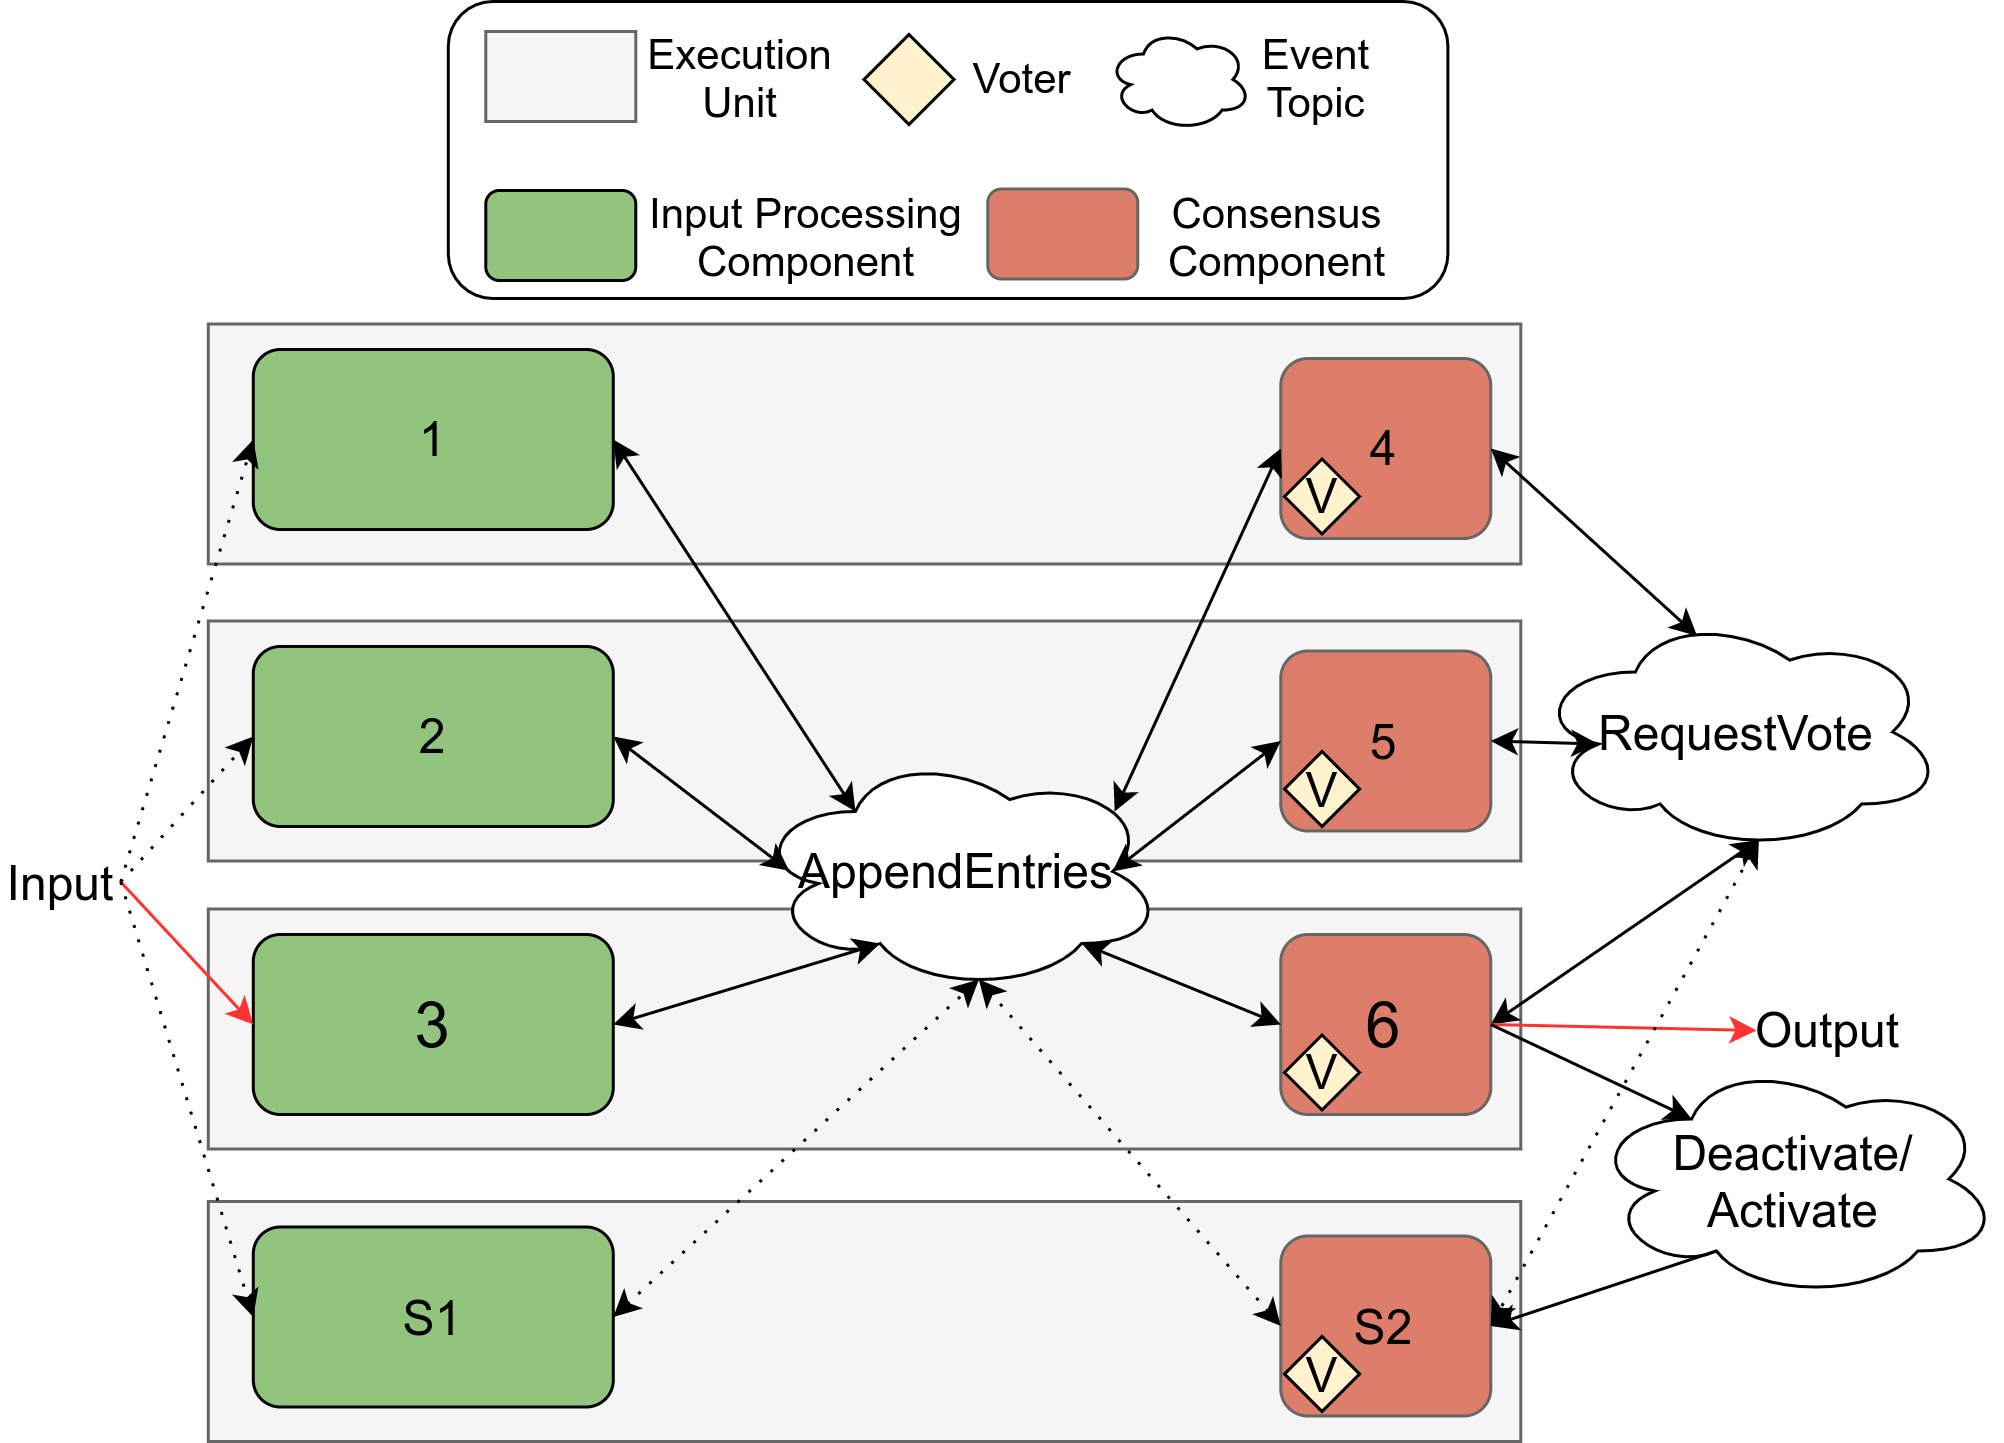
\includegraphics[width=0.9\linewidth]{images/ThreeEUConsensusDDS}
	\caption{A raft consensus algorithm requires at least two types of \glsentryfull{RPC} to be passed in the system, namely \texttt{RequestVote} and \texttt{AppendEntries}. These two can be implemented using \glsentryfull{DDS} event topics.}
	\label{fig:ThreeRepConsensusDDS}
\end{figure}

\autoref{fig:ThreeRepConsensusDDS} shows how the concept of \texttt{Raft}, with its roles and \abrpl{RPC}, can be implemented within a pipelined approach using \abr{DDS}.
In this example, the replicas of type (A) publish their intermediate results in a \abr{DDS} event topic, which can be read by the individual voters.
Replica (4) with its corresponding voter took over the leader role and thereby controls the system's output by performing a majority voting over the intermediate results.
In addition, the leader publishes periodic heartbeat messages to the \texttt{AppendEntries} topic, which are received by the followers (5) and (6).
When a heartbeat message stayed out for a period, the system assumes that the leader has crashed and the followers initiate a new leader election using the \texttt{RequestVote} topic.
When a new leader is elected, it gains complete control over the output, subscribes to the \texttt{Replica A Result} topic, and starts sending heartbeat messages.
In the event of the previous leader coming back online again, it subscribes to \texttt{AppendEntries}, receives heartbeat messages and thereby takes over a follower role.
Thereby, crash faults (\textbf{F1}) for voters can be caught by the heartbeat mechanism.

The implemented pipelined approach, as constituted in~\autoref{fig:ThreeRepConsensusDDS}, is deployed on three execution units for cost and space reasons.
Further, the input frequency for the applied use-case is small compared to the system's throughput whereby a \ChallengeThrough is no problem.
Nevertheless, the approach can be spread out to more replicas by distributing the logic modules accordingly.
This is because the connecting \abr{DDS} topics allow free arrangement of the solution's logic modules.
\\

In order for the application to notice available data samples, \texttt{WaitSets} are used.
\texttt{WaitSets} are preferred over \texttt{Listeners} because they are state-based rather than event-based, which means they trigger as long as a certain state is present rather than when an event is triggered.
Thereby, it can be ensured that no available data is missed.
Further, by using \texttt{WaitSets}, the entire control about the application is managed by the application itself and no application code is executed in middleware threads.
\\

The system's state is stored as a global state in \abr{DDS} state topics and thereby managed by the middleware.
This ensures that all replicas can operate on the most recent system state and no replica becomes outdated.
Only the system's leader is permitted to alter the system's state, all other replicas have read-only access.
\\

The consensus algorithm guarantees that there is at most one leader present in the system at a time - i.e. no split brain - and that a new leader is elected when there is none present.
Time in \texttt{Raft} is subdivided into \textit{terms}, that each start with a leader election.
Each replica manages its own term as a private replica state.
Besides the current term, the replicas current \texttt{Raft} role and voting information is organized in the replica's private state.
The private state is kept up to date by exchanging messages with other replicas.

\subsection{Leader Election}
\begin{figure}[!hb]
	\centering
	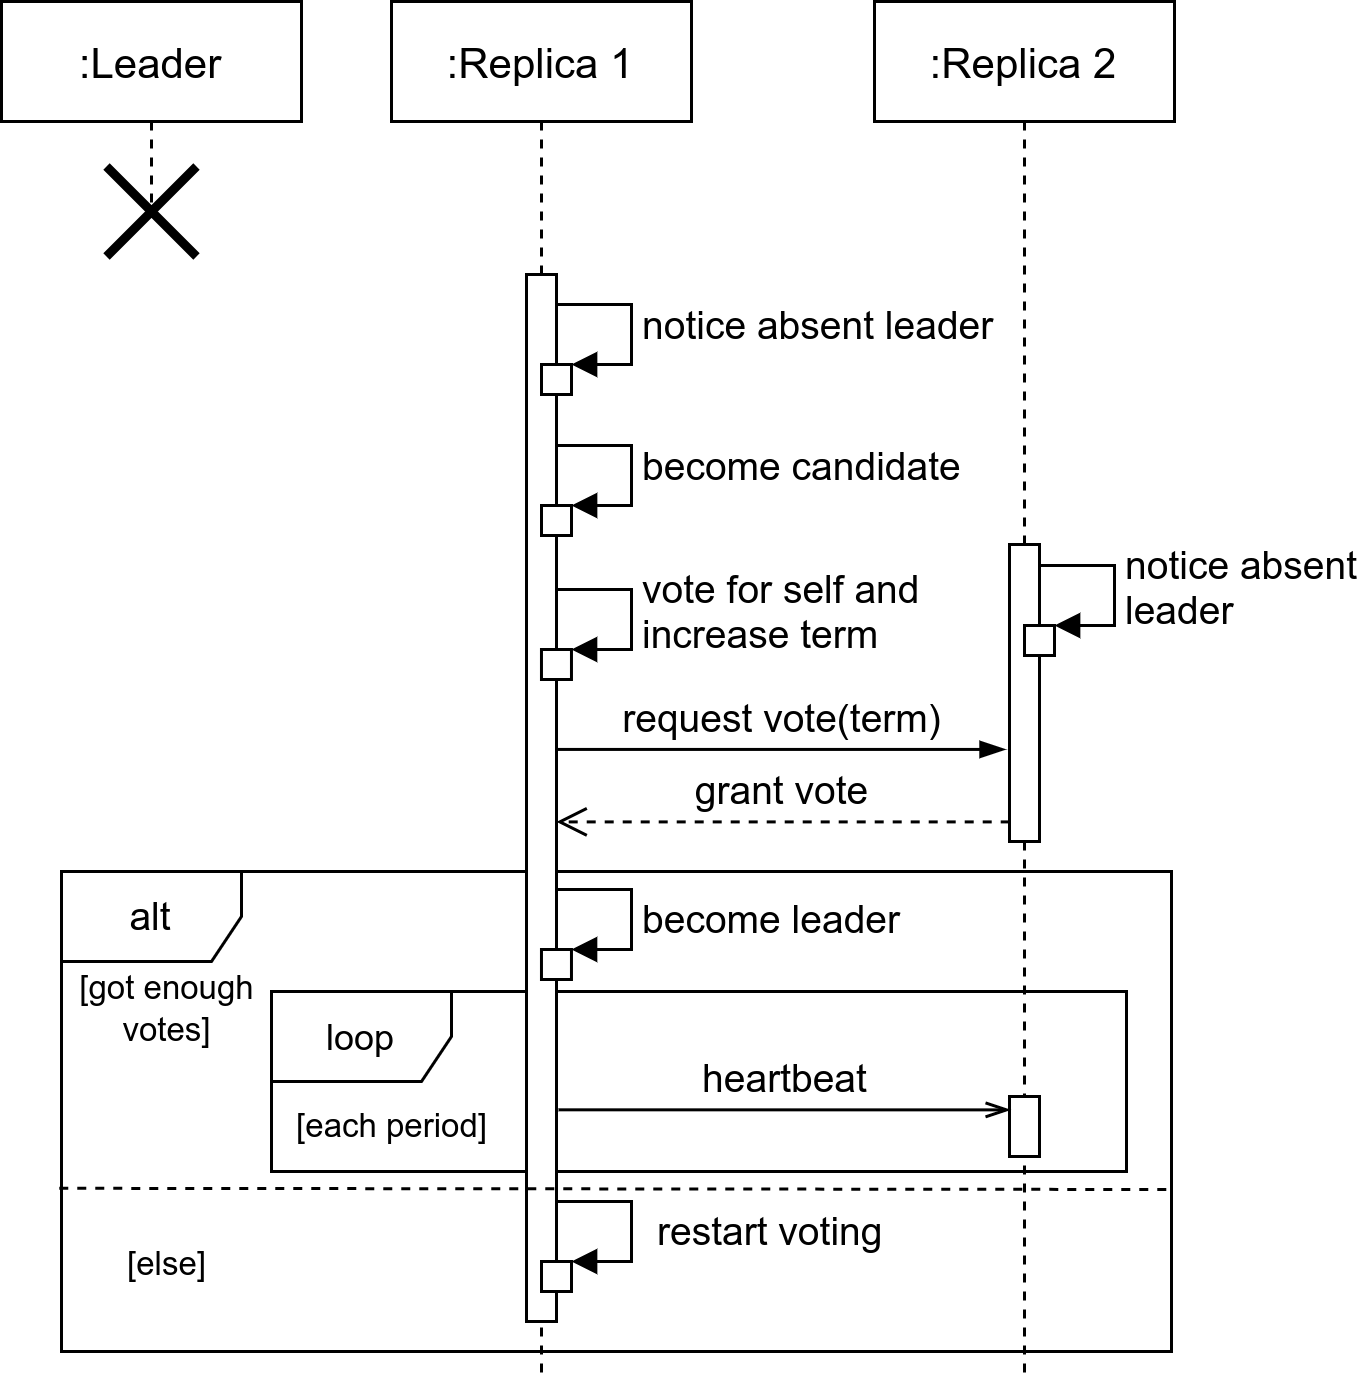
\includegraphics[width=0.75\linewidth]{images/sequence/LeaderElection}
	\caption{When a replica notices that the leader crashed, it becomes a candidate, votes for itself and sends vote requests to all remaining replicas. When enough votes were granted, it becomes the new leader and starts sending heartbeats. Otherwise, it retries to become leader in the next term.}
	\label{fig:SeqLeaderElection}
\end{figure}

The presence of a leader in the system is detected through heartbeat messages.
When a replica does not receive a message from a leader for a specific period of time, called the \textit{election timeout}, it tries to become leader by initiating the voting process.
A high level overview about the voting process, after the previous leader crashed, is depicted in~\autoref{fig:SeqLeaderElection}.
Replica 1 notices the crashed leader first and tries to become the new leader by switching into candidate mode and sending a vote request to each remaining replica.
In the exemplary case in~\autoref{fig:SeqLeaderElection}, replica 2 accepts the vote request and replica 1 becomes the new leader.
It immediately starts sending heartbeat messages afterwards.
\\
In the following, the allocation, as well as the collection of votes, will be discussed in more detail.
\\\\
\begin{algorithm}[H]
\caption{Algorithm for vote allocation. Whether a vote gets granted or rejected depends on whether the replica that receives the vote request has already voted for another replica in the current voting's term.}\label{algo:VoteAllocation}
\SetKwData{Term}{\textit{term}}
\SetKwData{Sender}{\textit{senderID}}
\SetKwInOut{Input}{input}
\SetKwInOut{Output}{output}

\Input{A vote request with a \Term and a \Sender}
\Output{true if the vote for \Sender in \Term was granted, false otherwise}
\BlankLine
\If{\Term $<$ current term}{become follower in new \Term\;}
\If{\Term $==$ current term \textbf{AND} not voted in current term}{grant vote for \Sender\;}
\end{algorithm}

The allocation of votes is shown in~\autoref{algo:VoteAllocation}.
Each replica can only vote for a single other replica in each term.
Because the system's state is managed globally by \abr{DDS}, every replica is equally up to data so that vote allocation is implemented in a first-come-first-serve manner.
As soon as a vote request is received that has a higher term number than the replica's term, is automatically transitions into the follower state, because the system will have a new leader in the new term.
\\\\
\begin{algorithm}[H]\caption{Algorithm for vote collection. Only votes that were answered in the same term that the vote request was issued are considered. When enough votes are collected, the replica becomes leader. If a votes was answered in a more recent term, the vote collection gets aborted and the replica becomes a follower.}\label{algo:VoteCollection}
\SetKwData{VoteTerm}{\textit{voteTerm}}
\SetKwData{VoteGranted}{\textit{voteGranted}}
\SetKwInOut{Input}{input}
\SetKwInOut{Output}{output}

\Input{A vote reply with a \VoteTerm and a \VoteGranted flag}
\Output{Transition to either leader or follower state}glsentryfull
\BlankLine

\If{the replica is no candidate anymore}{return\;}
\If{\VoteTerm $>$ term when election started}{
become follower\;
return\;}
\If{\VoteTerm $==$ term when election started \textbf{AND} vote got granted}{
Increase number of granted votes in the election term\;
	\If{got enough votes}{
	become leader\;
	return\;}
}
\end{algorithm}

Whether a vote requests gets accepted or declined depends on the request's data and the replicas private state.
For each vote reply that is received by a replica, it is first checked whether the replica has left the candidate state in the meantime, which makes the entire vote reply irrelevant.
This can, for example, happen when another vote request with a higher term number has been granted while the replica waits for incoming vote replies itself.
Afterwards it is checked whether the term in which the vote request got processed by another replica is higher than the term in which the voting was started.
This fact indicates that the corresponding replica is outdated, so that it transitions into follower state and should not become a leader in the regarded voting process.
Finally, when the vote got granted and enough granted votes were received, the replica is elected as a new leader for the corresponding term.
The number of necessary voted depends on the total number of replicas in the system.

\begin{figure}[!hb]
	\centering
	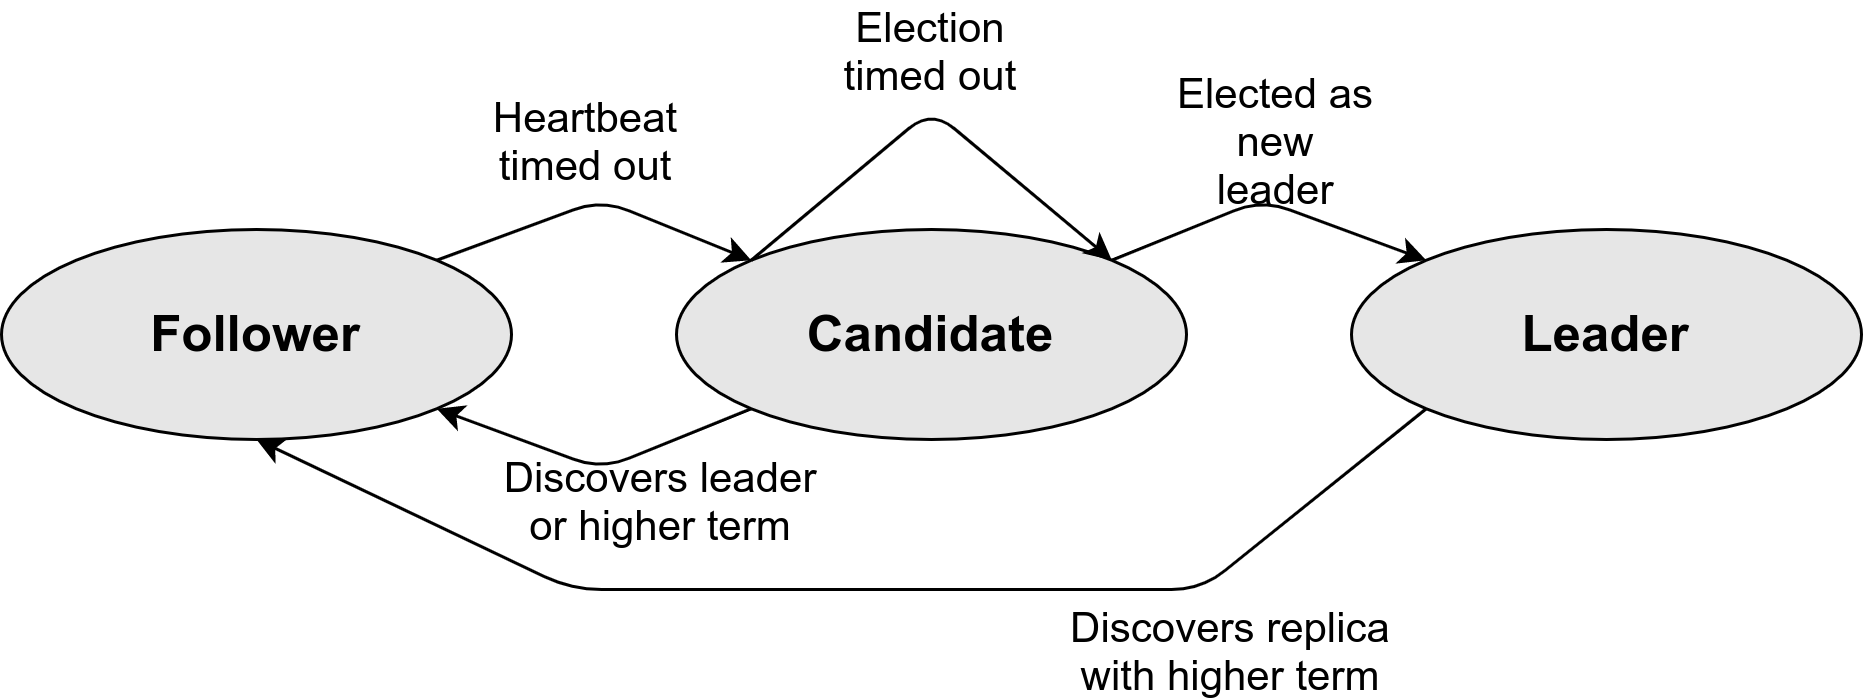
\includegraphics[width=0.75\linewidth]{images/RaftServerStates}
	\caption{Taken from~\cite{RaftConsensusPaper}. Replicas in \texttt{Raft} can be in one of three states. When a follower receives no message from a leader, it starts an election and tries to become the new leader. Leaders operate until they fail or until they discover that their term is outdated.}
	\label{fig:RaftServerStates}
\end{figure}

During the entire time, each replica is in one of three states, namely \texttt{Leader}, \texttt{Candidate} or \texttt{Follower}.
The leader election process can be summarized as transitions and corresponding conditions between these three states, as depicted in~\autoref{fig:RaftServerStates}.
Five requirements can be derived from the figure that must be met by an algorithm that implements \texttt{Raft}'s leader election process:

\begin{enumerate}
\item \textbf{Start Election:} A follower becomes candidate, increments its term, votes for itself and sends a message to all other replicas stating that it wants to become leader.
\item \textbf{End of Election:} A candidate remains in candidate state until it either wins the election, receives information about another leader in the system, or times out.
\item \textbf{Won Election:} A candidate wins the election if it receives votes from a majority of replicas in the same term. Each replica votes for at most one replica in a given term.
\item \textbf{Lost Election:} When a candidate receives a message from a leader in the system and the leader's term is at least as high as the candidate's term.
\item \textbf{No Result:} A certain period of time goes by without the candidate winning or loosing the election.
\end{enumerate}
In the following, it is described how these requirements are met by using \abr{DDS} features.
Thereby, the functional correctness of the transcribed leader election algorithm is proven.

\lstset{language=C}
\begin{lstlisting}[caption={\abr{IDL} definition for the \texttt{AppendEntries} topic. The \texttt{term} variable represents the latest term that the replica has seen, while the \texttt{senderID} encodes which replica sent this message. With \texttt{entries}, a payload can be send via the topic. This is used by a leader for instructing its followers to process certain data. The \texttt{entries} field is left empty for heartbeat messages.}, label=code:appendEntries]
struct AppendEntries {
    long term;
    long senderID;
    sequence<Entry> entries;
};
#pragma keylist AppendEntries term
\end{lstlisting}

\begin{lstlisting}[caption={\abr{IDL} definition for the \texttt{RequestVote} topic. The \texttt{term} variable represents the candidate's term, while \texttt{candidateID} encodes the candidate that requested the vote.}, label=code:requestVote]
struct RequestVote {
    long term;
    long candidateID;
};
#pragma keylist RequestVote
\end{lstlisting}

\begin{lstlisting}[caption={\abr{IDL} definition for the \texttt{RequestVoteReply} topic. The \texttt{term} encodes the sender's term for the candidate to update itself. \texttt{voteGranted} shows whether the replica granted the vote request for the given term. The \texttt{candidateID} and \texttt{senderID} are used to identify which replica granted the vote for which replica respectively.}, label=code:requestVoteReply]
struct RequestVoteReply {
    long senderID;
    long term;
    long candidateID;
    long voteGranted;
};
#pragma keylist RequestVoteReply
\end{lstlisting}

For realizing the leader election algorithm with \abr{DCPS} features, three \texttt{Topics} are required.
The \texttt{AppendEntries} and \texttt{RequestVote} topics are representatives for the corresponding \texttt{Raft} \abrpl{RPC}.
The \abr{IDL} representation for \texttt{AppendEntries} is shown in~\autoref{code:appendEntries}.
In accordance to that, \texttt{RequestVote} is represented by a topic whose \abr{IDL} is shown in~\autoref{code:requestVote}.
Because data objects that are managed by \abr{DDS} require a predetermined structure, a dedicated topic for replying to vote requests is required.
Therefore, \texttt{RequestVoteReply} is utilized as described in~\autoref{code:requestVoteReply}.

For implementing an \textit{election timeout}, a \texttt{WaitSet} with a corresponding \texttt{ReadCondition}, that triggers when new data has been published to \texttt{AppendEntries}, is applied.
Although a heartbeat message is a periodic message and a deadline \abr{QOS} could be used to register an absent leader, a timeout attached to a \texttt{WaitSet} is preferred.
This is because a \texttt{WaitSet} with a timeout is required for other messages as well and the deadline \abr{QOS} would require a \texttt{StatusCondition} to be noticed whereby the utilized \abr{DDS} subset would grow.
In order to initiate the voting process, the replica publishes a new vote request to \texttt{RequestVote}.
Because the middleware ensures that data is transmitted to all replicas that subscribed to a topic, the \textbf{Start Election} requirement can easily be solved with \abr{DDS}.

Further, \textbf{No Result} can be resolved by using a \texttt{WaitSet}, called \textit{leaderElection\_WaitSet}, with a corresponding timeout (\textit{leader ready timeout}).
When the timeout expires, the replica starts to wait for heartbeat messages again.
In addition to the timeout, a \texttt{ReadCondition} is attached to the \textit{leaderElection\_WaitSet} that triggers when messages from a leader have been published to the \texttt{AppendEntries} topic.
Thereby, \textbf{Lost Election} is ensured.
By implication, this means that the candidate either won the election, or the election was not successful for the turn, when the timeout attached to \textit{leaderElection\_WaitSet} expires.

However, because each replica waits for incoming heartbeats after it won the election, a leader could simultaneously read its own heartbeats.
This is because each replica has simultaneously registered a \texttt{DataWriter} and \texttt{DataReader} to each topic.
Therefore, after reading each data sample, the application code must manually verify that the message was not published by the same replica that is reading the message by comparing its identification number with the received \textit{senderID}.
Because it depends on the replica's role whether it should publish or subscribe to a topic and each replica could become the leader or a follower at any point in time, all \abr{DDS} entities and subscriptions are set up during application initialization.
Thereby, time is saved during role reversal.
On the other hand, this also has the effect that each replica has \texttt{DataReaders} that receive messages published by \texttt{DataWriters} from the same replica.
While \texttt{QueryConditions} could be used to solve this by filtering messages, \texttt{ReadConditions} have been used because it ensures that each data sample is read and \texttt{DataReaders} with resource limit \abr{QOS} settings are not overfilling.
This partly solves \textbf{Won Election}.

In order to fully solve \textbf{Won Election}, each replica needs to collect votes and reply to vote requests, parallel to detecting other leaders and voting timeouts.
The voting part is therefore treated by another \abr{OS} thread, that again makes use of a \texttt{WaitSet}, where two \texttt{QueryConditions} are attached to, one for the \texttt{RequestVote} and one for the \texttt{RequestVoteReply} topic.
Thereby, the replicas can come to an agreement about a vote request while the candidate waits for the voting to end.

\subsubsection{Race Conditions}
\begin{figure}[!hb]
	\centering
	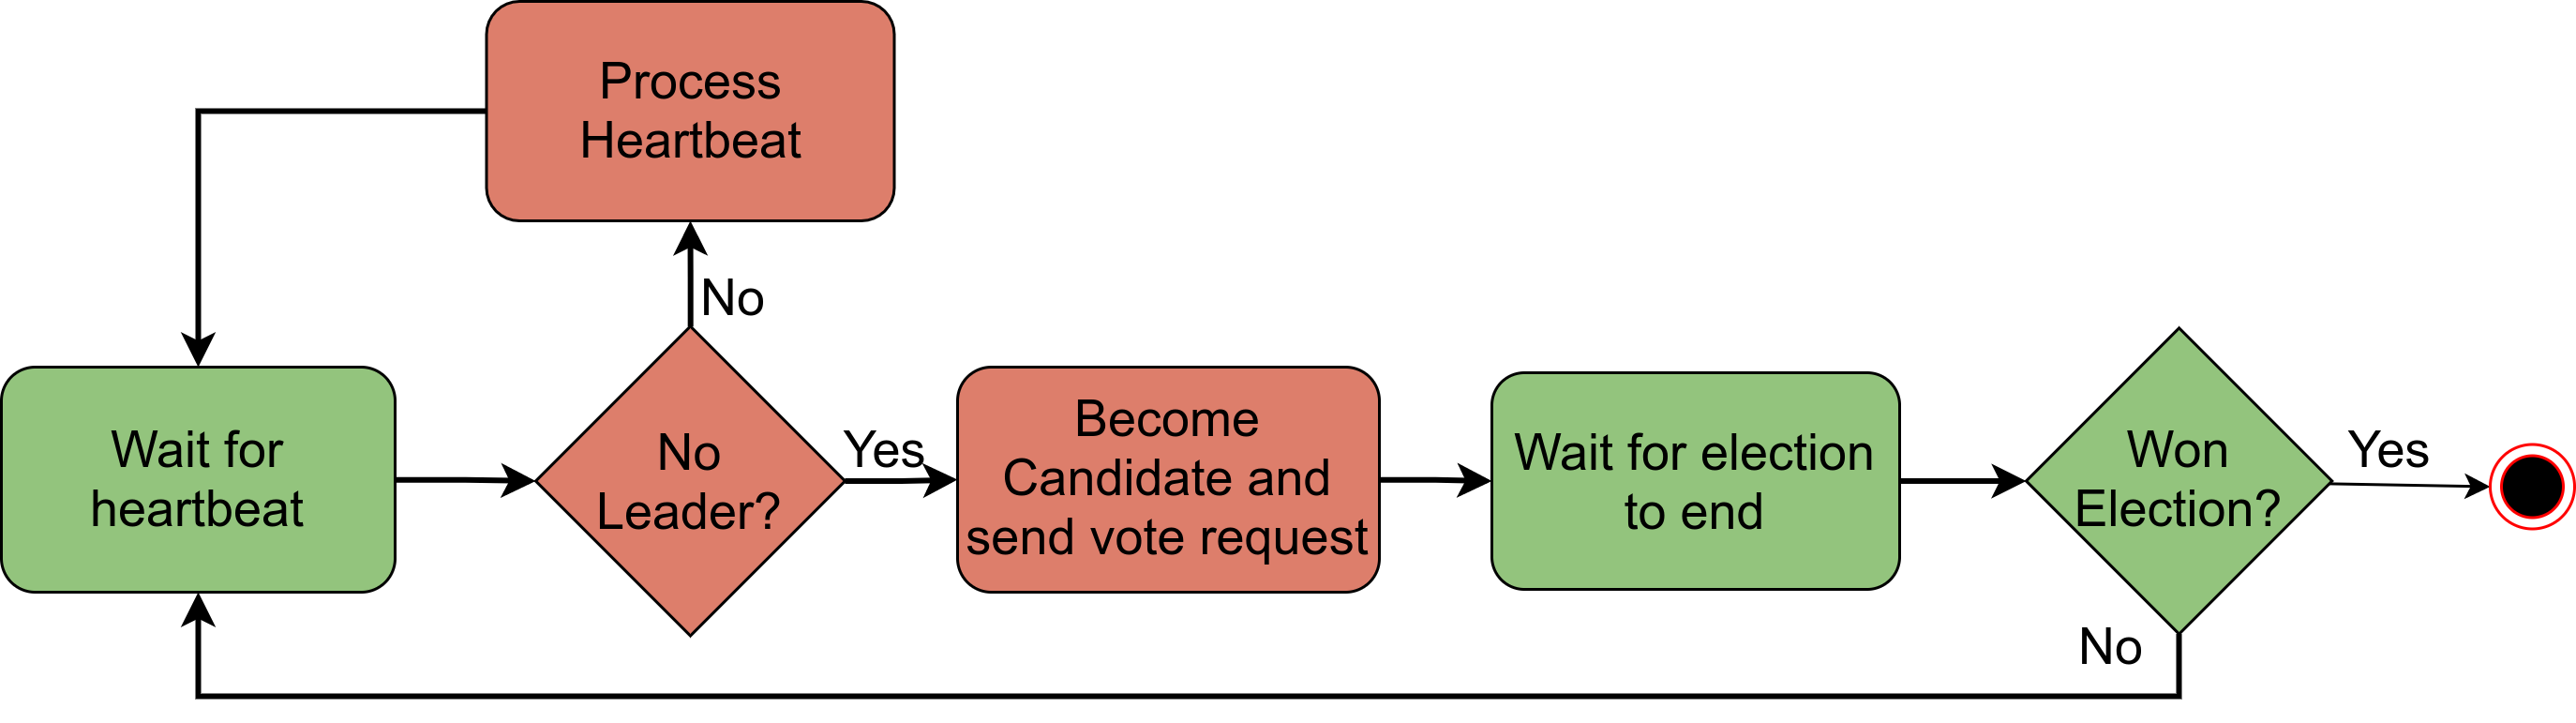
\includegraphics[width=0.75\linewidth]{images/LeaderElectionHeartbeatThread}
	\caption{One \glsentryfull{OS} thread of the leader election process is the "Heartbeat Thread". In this thread, followers receive \texttt{AppendEntries} messages from leaders and detect missing leaders through expiring timeouts. The thread also initiates the voting process by sending an initial vote request. A mutex ensures that the algorithm can only be preempted before or after a part that is depicted in green. Consecutive red parts are executed atomically.}
	\label{fig:LeaderElectionHeartbeatThread}
\end{figure}

\begin{figure}[!hb]
	\centering
	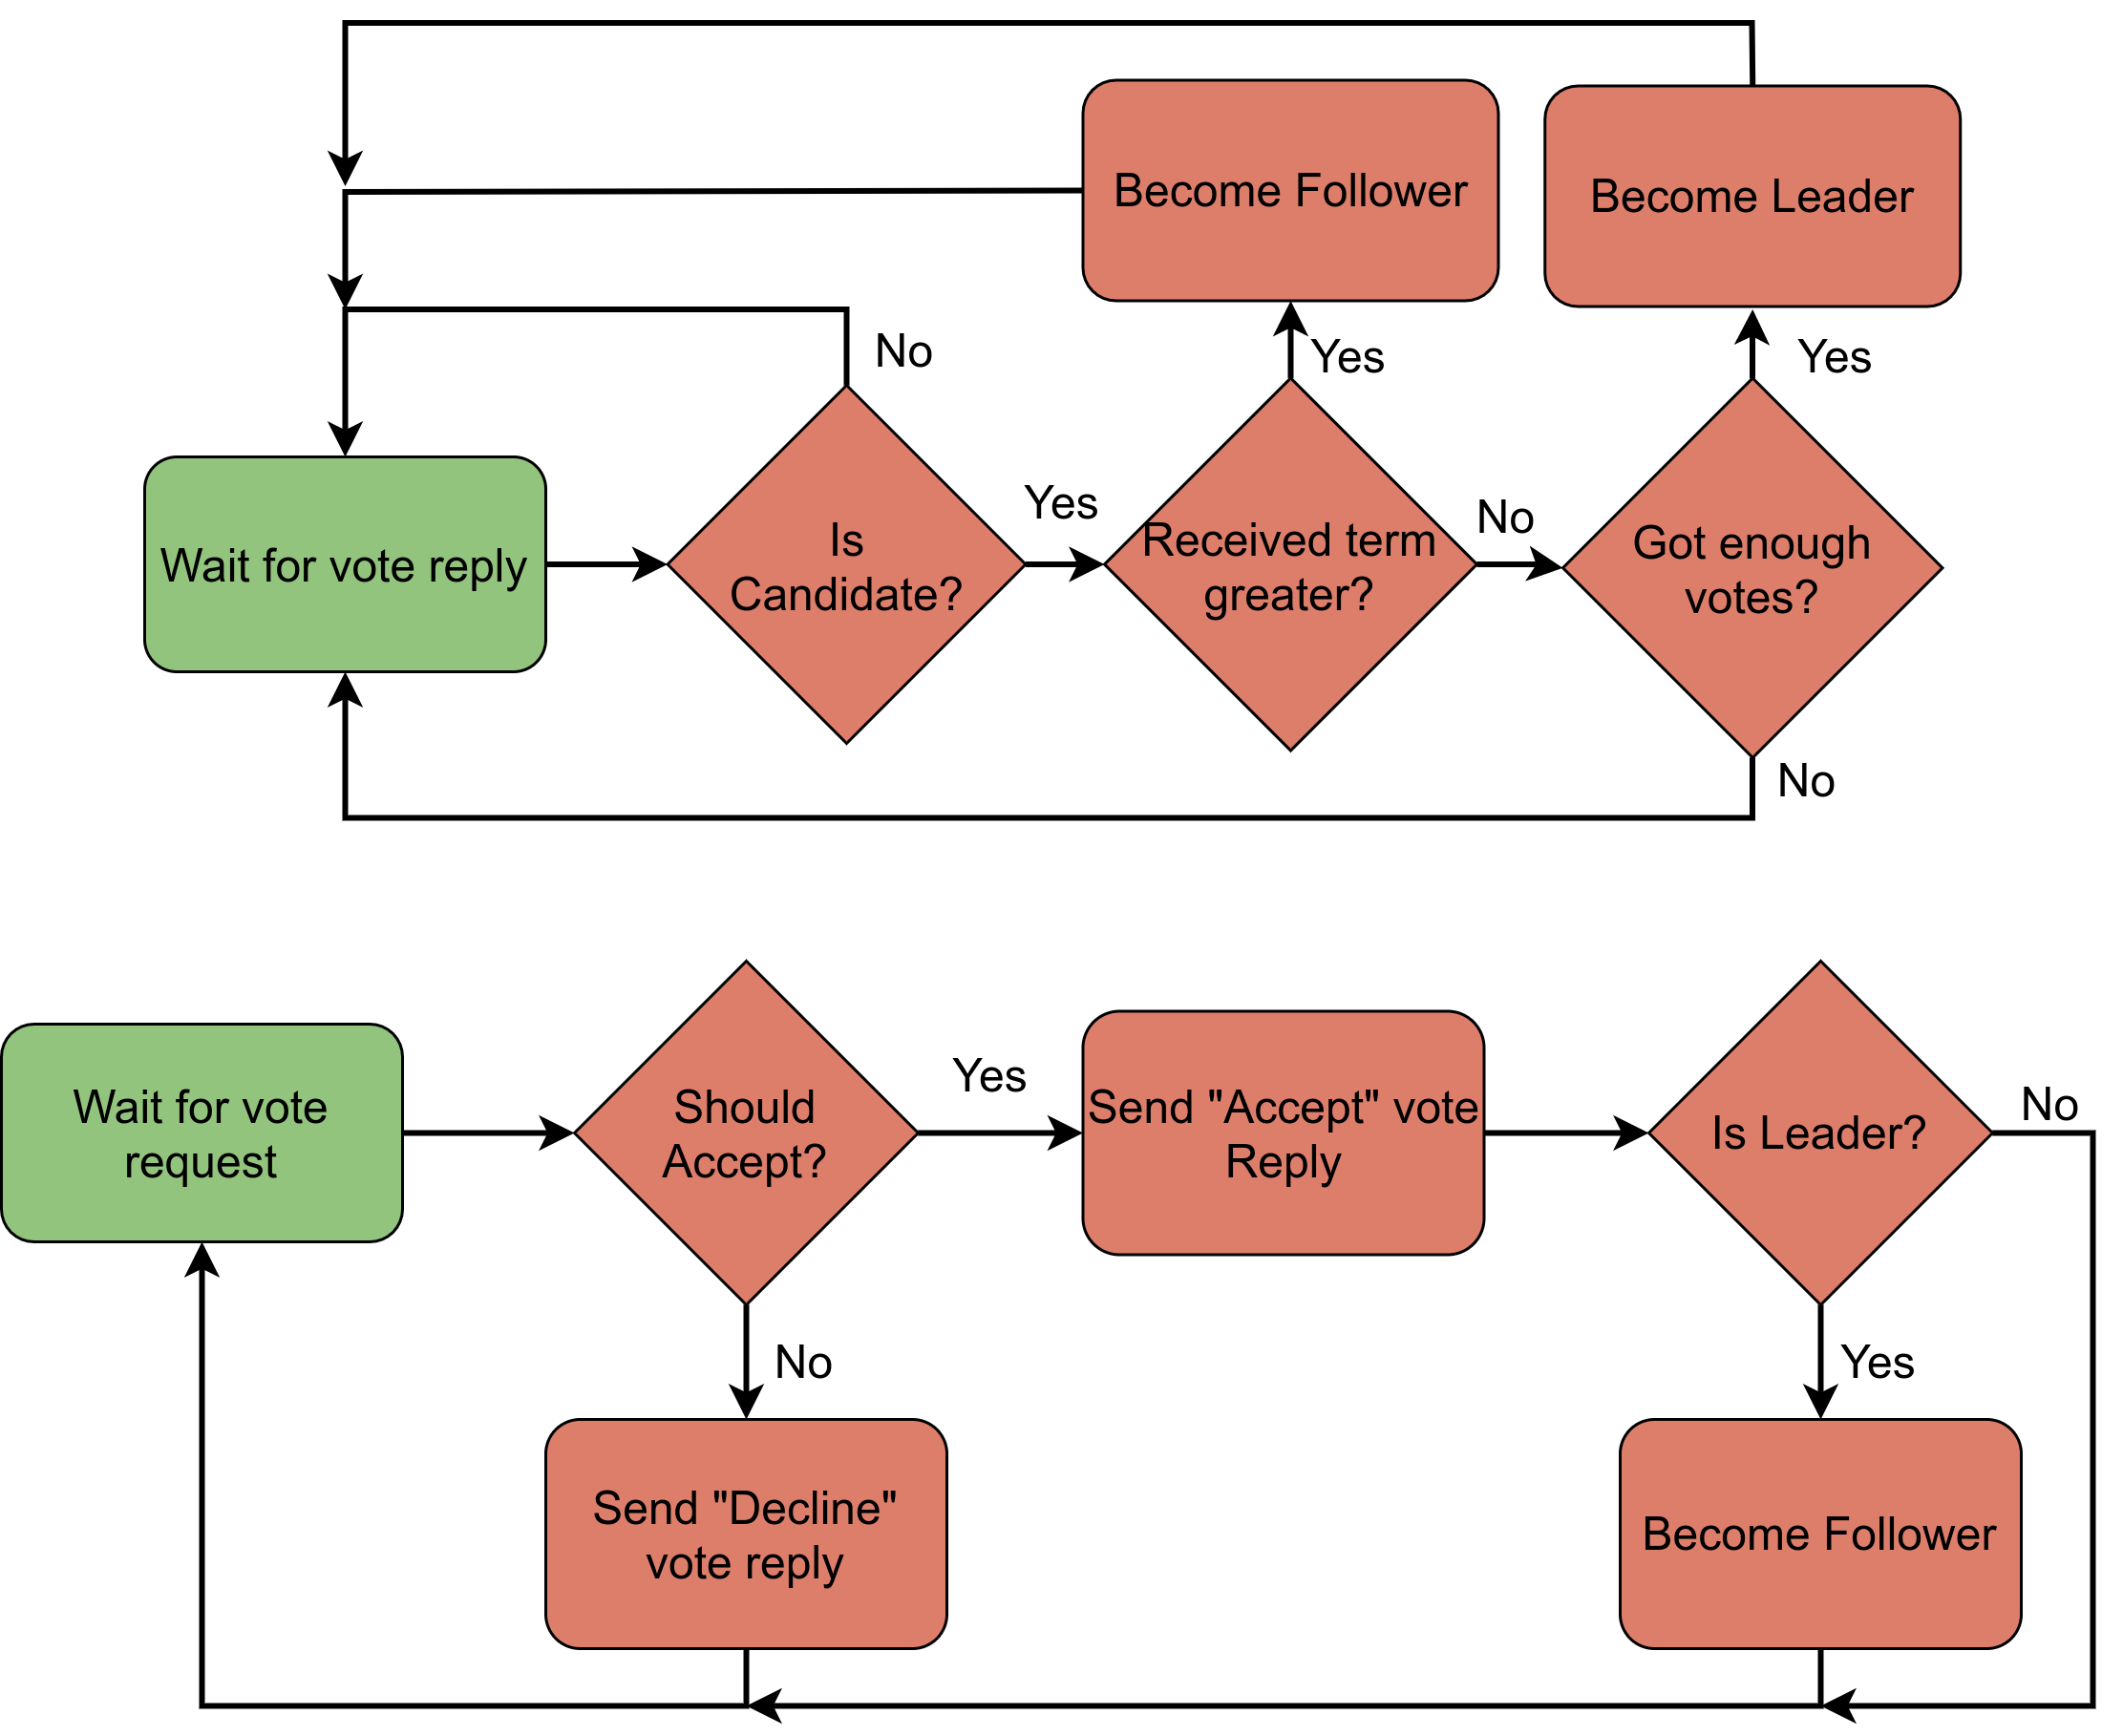
\includegraphics[width=0.75\linewidth]{images/LeaderElectionVoteThread}
	\caption{One \glsentryfull{OS} thread of the leader election process is the "Vote Thread". In this thread, replicas respond to vote requests and handle replies they got for their own vote requests. A replica's action to the requests depends on their private state. A mutex ensures that the algorithm can only be preempted before or after a part that is depicted in green. Consecutive red parts are executed atomically.}
	\label{fig:LeaderElectionVoteThread}
\end{figure}

The leader election algorithm is structured into three parts which are executed on two \abr{OS} threads.
One part is the processing of heartbeat messages in a "Heartbeat Thread, as depicted in~\autoref{fig:LeaderElectionHeartbeatThread}.
In the "Heartbeat Thread", each follower listens for heartbeat messages and start a leader election process by sending vote requests when the corresponding timeout expires.
The other two parts, namely answering vote requests, and processing replies to vote requests, are handled in another thread and are depicted in~\autoref{fig:LeaderElectionVoteThread}.
Since the program is structured as a multi-threaded concurrent system that is required to make decision based on the replica state and no assumptions about the thread's relative speed can be made, race conditions can occur~\cite{Dijkstra1965}.
Replica internal race conditions are prevented by utilizing a mutex in order to ensure that its private state, including the replica's \texttt{Raft} role, the current term, and voting information, does not change while answering a message.
Race conditions among replicas are prevented though a history \abr{QOS}-policy and a continuously increasing term number.
The history \abr{QOS}-policy ensures that new requests are buffered in a \texttt{DataReader} while another is processed.
This ensures that no request is neglected.
Further, a continuously increasing term number enables the system to detect outdated requests or recognize when the replica itself is outdated.


\subsubsection{Time Considerations}
\label{subsub:timeConsiderations}
Because each \texttt{WaitSet} in \abr{DDS} can be attached with a timeout, the maximal time that the system is without a leader can be determined.
This is further measured and analyzed in~\autoref{chptr:evaluation}.
There are two timeouts involved in the leader election process, namely the \textit{election timeout}, whereby a missing leader is elected, and the \textit{leader ready timeout}.
When the \textit{leader ready timeout} expires, it was impossible for the system to elect a new leader for the given term.
This can, for example, happen due split votes when multiple followers try to become the new leader at the same time, or because there are not enough active replicas in the system.
The proposal that \texttt{Raft} makes to reduce the risk of split votes is to use randomized \textit{election timeouts}.
However, this does not prevent split votes from happen at all.
Therefore, in this implementation, the \textit{election timeout} is made directly dependent on the replicas unique identification number, so that they never try to become leader at the same time.
Although replicas with certain identification numbers are thereby preferred in the leader election process, this approach is not a disadvantage because, due to \abr{DDS}'s global data space, no replica is ever more suitable for becoming the new leader than some other.
Further, a replica with an outdated term number is still excluded from becoming a leader because their vote requests would get declined.

On the other hand, network delays or too few active replicas are safety risks and should be dealt with accordingly.
For doing so, a maximal time that the system should be without a leader can be specified.
Altogether, when enough replica are present in the system and communication is possible without any delays, the system will not be without a leader for the maximum time of $\textit{election timeout} + \textit{leader ready timeout}$.

\subsection{Input Processing}
\todo{Describe in more detail like the leader election}
\label{subsec:ImpInputProcessing}
\begin{figure}[!hb]
	\centering
	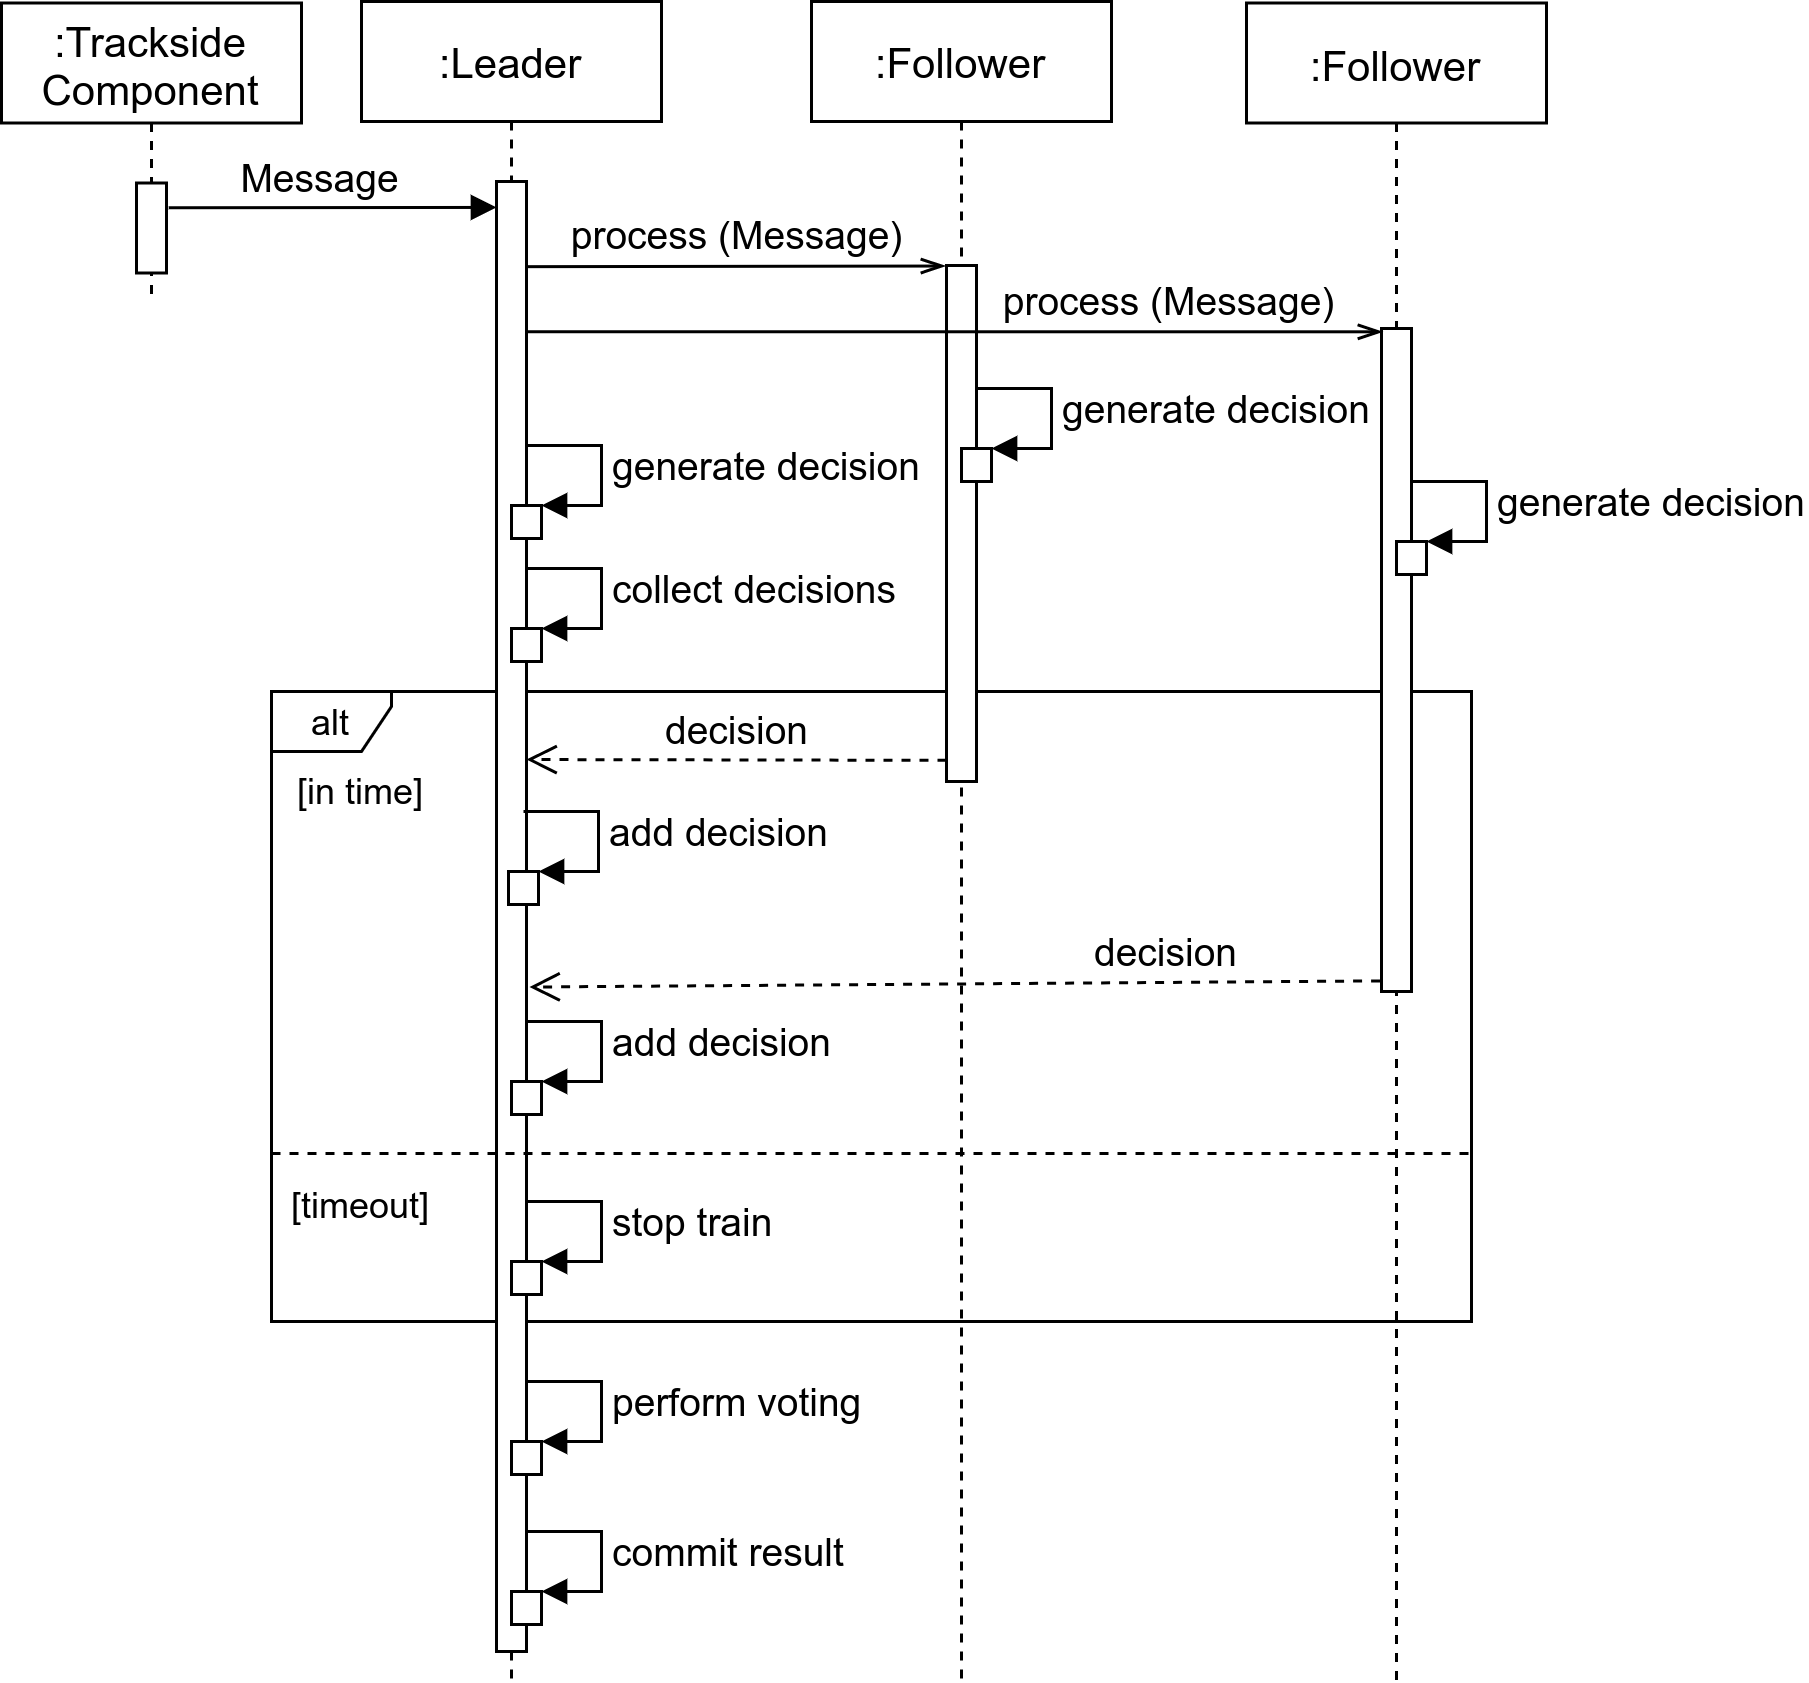
\includegraphics[width=0.75\linewidth]{images/sequence/CollectResults}
	\caption{Input messages from track-side components are recorded by the leader and replicated to its followers. Afterwards, the leader and each follower process the input and generate a decision based on the data and the global system state. The decisions are collected by the leader and a voting is performed on the collected decisions. Meanwhile, the leader ensures that time constraints are met using timeouts.}
	\label{fig:SeqCollectResults}
\end{figure}

The purpose of the established redundant application is to process input messages from \abr{RBC} and track-side components and generate a single reaction on the input for the entire system based on majority voting.
A coarse overview about how input messages are distributed among the replicas and processed by the system is presented in~\autoref{fig:SeqCollectResults}.
It is the leaders responsibility to record new inputs, replicate the inputs to each follower, maintain the system's global state, and generate a final outpur to each input.
All communication among the replicas takes place via \abr{DDS}.
As soon as the leader receives an input messages, it starts to assign each follower to process the input.
This is done through the \texttt{AppendEntries} topic and follows the log replication process from \texttt{Raft}.
Afterwards, all replicas are generating a decision for the input message in parallel based on the global system state which is managed by \abr{DDS}.
The followers publish their decisions on the \texttt{AppendEntriesReply} topic.
When the leader has made its decision, it starts collecting the follower's decisions using a \texttt{WaitSet} and a \texttt{QueryCondition} on the \texttt{AppendEntriesReply} topic.
A timeout is attached to this \texttt{WaitSet} to ensure that, after a certain time-span, the voting process can start based on all results that reached the leader at that time.
The leader performs a majority voting on all collected replica decisions and thereafter commits the final decision.
During the commit phase, all changes that the input messages has on the system's state are applied to the global data space.
Thereby, the decisions for all replicas are deterministic because they are all based on the same system state.
Furthermore, the input message is marked as processed during the commit phase by disposing its corresponding \abr{DDS} instance.
This ensures that, if the leader crashed while processing the input message, a new leader recognizes the input messages as unprocessed and restarts its processing.

The tasks required to successfully complete the scenario are fulfilled as follows:

\begin{itemize}
\item The leader accepts linking and \abr{MA} information and incorporates them into the global system state
\item The system updates the train's position and confidence interval with every heartbeat message
\item The leader periodically initiates a braking curve analysis and comparison with the current \abr{MA}
\item After reading a balise telegram message, the leader distributes it across the system and performs a voting whether the train should brake or continue driving
\end{itemize}

\subsection{State Manager}
\todo{Describe in more detail like the leader election}

\begin{lstlisting}[caption={\abr{IDL} definition for the \texttt{LinkedBalises} topic. Each linked balise has an unique identifier and a position that is communicated to the system by the \abr{RBC}.}, label=code:linkedBalises]
struct LinkedBalises {
    short ID;
    long position;
};
#pragma keylist LinkedBalises ID
\end{lstlisting}

\begin{lstlisting}[caption={\abr{IDL} definition for the \texttt{MovementAuthority} topic. The \texttt{start\_position} encodes where the \abr{MA} starts and the \texttt{end\_position} encodes until where it is valid.}, label=code:movementAuthority]
struct MovementAuthority {
    long start_position;
    long end_position;
};
#pragma keylist MovementAuthority
\end{lstlisting}

\begin{lstlisting}[caption={\abr{IDL} definition for the \texttt{TrainState} topic. The train's state consists of a current position and a current speed. Due to inaccuracies of the position sensors, a train's position cannot be determined exactly. Therefore, a confidence interval is maintained that defines an area where the train certainly is. This area is bounded by \texttt{max\_position} and \texttt{min\_position}. With \texttt{is\_driving} it is encoded whether the virtual train drives or stands still. The \texttt{lastUpdateTime} variable is used to simulate the train's position based on its speed.}, label=code:trainState]
struct TrainState {
    double position;
    double max_position;
    double min_position;
    float speed;
    boolean is_driving;
    unsigned long long lastUpdateTime;
};
#pragma keylist TrainState
\end{lstlisting}
\todo{Trainstate driving in text}

It is mandatory for the replicas in the distributed system to produce deterministic results and to have access to the most recent global system state.
The global system state consists, inter alia, of the current \abr{MA} and a set of linked balises.
Although the train's position and speed are typically administered by other dedicated components in actual operation, they are simulated for the demonstrated system and therefore part of its global system state.
\\

\abr{DDS} can be used to manage the system's global state and ensure that any change is reliably trasmitted to all replicas.
Three \texttt{Topics} are used, namely \texttt{LinkedBalises}, \texttt{MovementAuthority}, and \texttt{TrainState}.

The \abr{IDL} representation for the \texttt{LinkedBalises} topic is shown in~\autoref{code:linkedBalises}.
Multiple balise instances can be stored within the topic that are distinguished by a unique identification number.
Since a set of linked balises is sent before journey and is not expected to change afterwards, an enduring \abr{DDS} state topic is used (see~\autoref{tab:stateQOS}).

The currently valid \abr{MA} is stored in the \texttt{MovementAuthority} topic, whose \abr{IDL} is shown in~\autoref{code:movementAuthority}.
As with the \texttt{LinkedBalises} topic, a movement authority is assigned once and valid for an entire journey so that it is stored in an enduring state topic.
Only one \abr{MA} is expected to be stored in the topic at any time.

The train's position and speed are stored in the \texttt{TrainState} topic, whose \abr{IDL} is shown in~\autoref{code:trainState}.
Three variables are used for the position.
One encodes the estimated position (\textit{position}) and two delimit an interval, the so called confidence interval, that certainly contains the train's true position.
A confidence interval is required because position measuring instruments can have inaccuracies.
The topic further contains a \texttt{is\_driving} variable that indicates whether the train moves or stands still and a \textit{lastUpdateTime} variable that determines when the position was updated for the last time.
This \texttt{lastUpdateTime} variable is only used for simulation reasons.
Because the state data is updated periodically and frequently, it should be managed as a volatile \abr{DDS} state topic.
\\

The topic's data is read and written like any other \abr{DDS} topic.
However, when a train starts a new journey and the new track section's linked balises have identification numbers that correspond with identification numbers of linked balises from previous track sections, special treatment is required.
In order to circumvent this situation beforehand, any data on the \texttt{LinkedBalises} topic is disposed before new data is written.

\section{Scenario Simulation}
\label{subsec:ScenarioSimulation}
\begin{figure}[!hb]
	\centering
	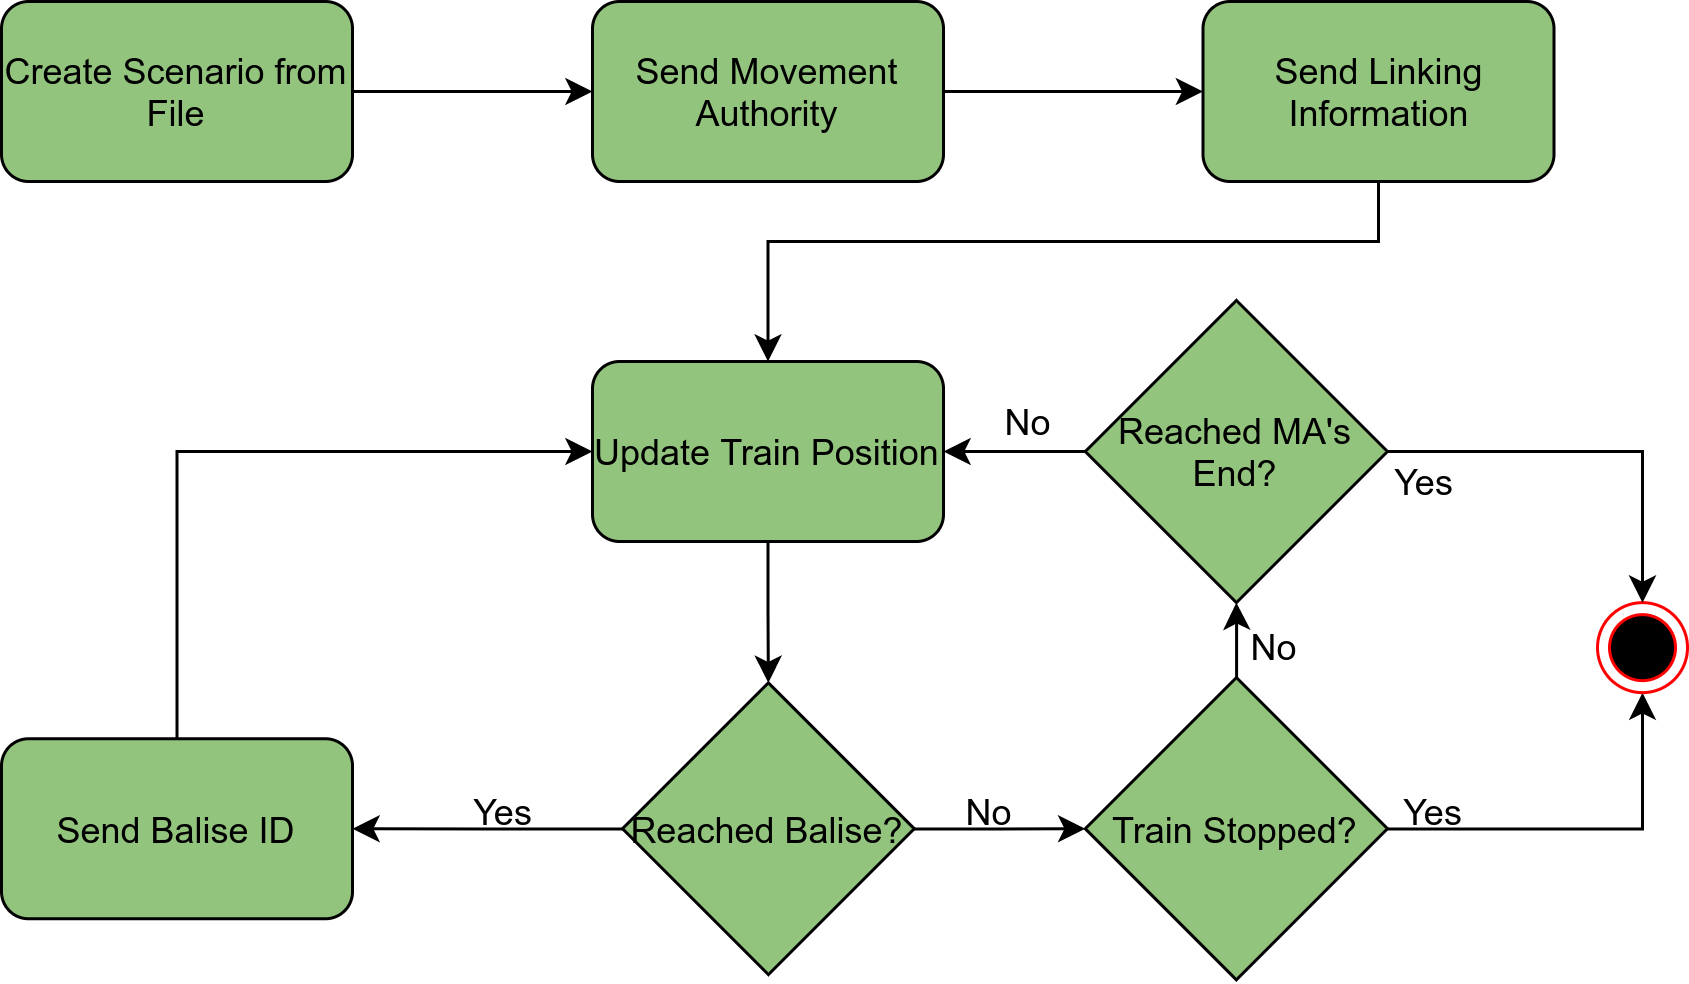
\includegraphics[width=0.75\linewidth]{images/SimulatorWorkflow}
	\caption{The scenario simulation's workflow. Each simulation begins by creating a scenario from a file and sending \glsentryfull{MA} and linking information. Thereupon, the virtual train is set in motion and balise telegrams are send on its way. When the virtual train stops early or when the \abr{MA}'s end is reached, the simulation stops.}
	\label{fig:SimulatorWorkflow}
\end{figure}
In order to demonstrate and evaluate the system's applicability, the \abr{ETCS} subset from~\autoref{sec:ImpScenarioDescription} is wrapped in a scenario and simulated.
The \abr{ETCS} subset consists of a \abr{MA} and a list of balises that function as positional landmarks.
Thus, a simulated scenario is bounded by a \abr{MA}'s start- and end-position and consits of one or multiple balises.
A simulated scenario's workflow is depicted in~\autoref{fig:SimulatorWorkflow}.

\begin{lstlisting}[caption={A JSON scenario representation. Each scenario consists of a \glsentryfull{MA} with a start and end point, as well as of a set of balises. Balises can be either linked or not and consist of an identification number, a linking position and an actual position. The linking position is transmitted to the on-board unit and is distinguished from its actual position to simulate a misplaced balise.}, label=code:scenarioJSON]
{
  "MA": {
    "start": 0,
    "end": 10
  },
  "balises": {

    "balise": {
      "id": 0,
      "link_pos": 1,
      "pos": 1,
      "linked": true
    },
    "balise": {
      "id": 1,
      "link_pos": 5,
      "pos": 5,
      "linked": true
    },
    "balise": {
      "id": 2,
      "pos": 7,
      "linked": false
    }

  }
}

\end{lstlisting}

At first, a scenario is created from a \textit{json} file.
An exemplary scenario in \textit{json} format is shown in~\autoref{code:scenarioJSON}.
It contains a \abr{MA} that starts at the current position and is valid for 1000 meters.
Further, three balises are simulated on the way, one at 100 meters, one at 500 meters, and one at 700 meters after the journey's start.
The first two balises will be linked with the on-board unit while the third will not.
Any linked balise further has a linking position field which is communicated to the on-board unit.
The distinction between a balise's actual position and its linking position is used to simulate balise that are not where they should be.
\\

After the \abr{MA} and the two linked balises have been sent to the on-board unit, the simulator starts to simulate a trip by updating the virtual train's position.
The position is continuously compared to the balise's positions and the \abr{MA}'s end.
As soon as the simulated train passes a balise's position, the corresponding balise is send.
In case that the balise lead to a braking action, for example because the balise was not linked or its position and linking position do not correspond, the simulation stops.
Finally, when all balises are evaluated successfully, the simulation ends when the \abr{MA}'s end is reached.

\section{Hot Standby}
\begin{lstlisting}[caption={\abr{IDL} definition for the \texttt{ActivateSpare} topic. This topic is used to activate or deactivate spare replicas. The \texttt{term} field encodes the term in which the activate or deactivate call has been made and \texttt{activate} gets interpreted as a boolean that encodes whether the spare should be activated or deactivated.}, label=code:activateSpare]
struct ActivateSpare {
    long term;
    long activate;
};
#pragma keylist ActivateSpare
\end{lstlisting}

\begin{figure}[!hb]
	\centering
	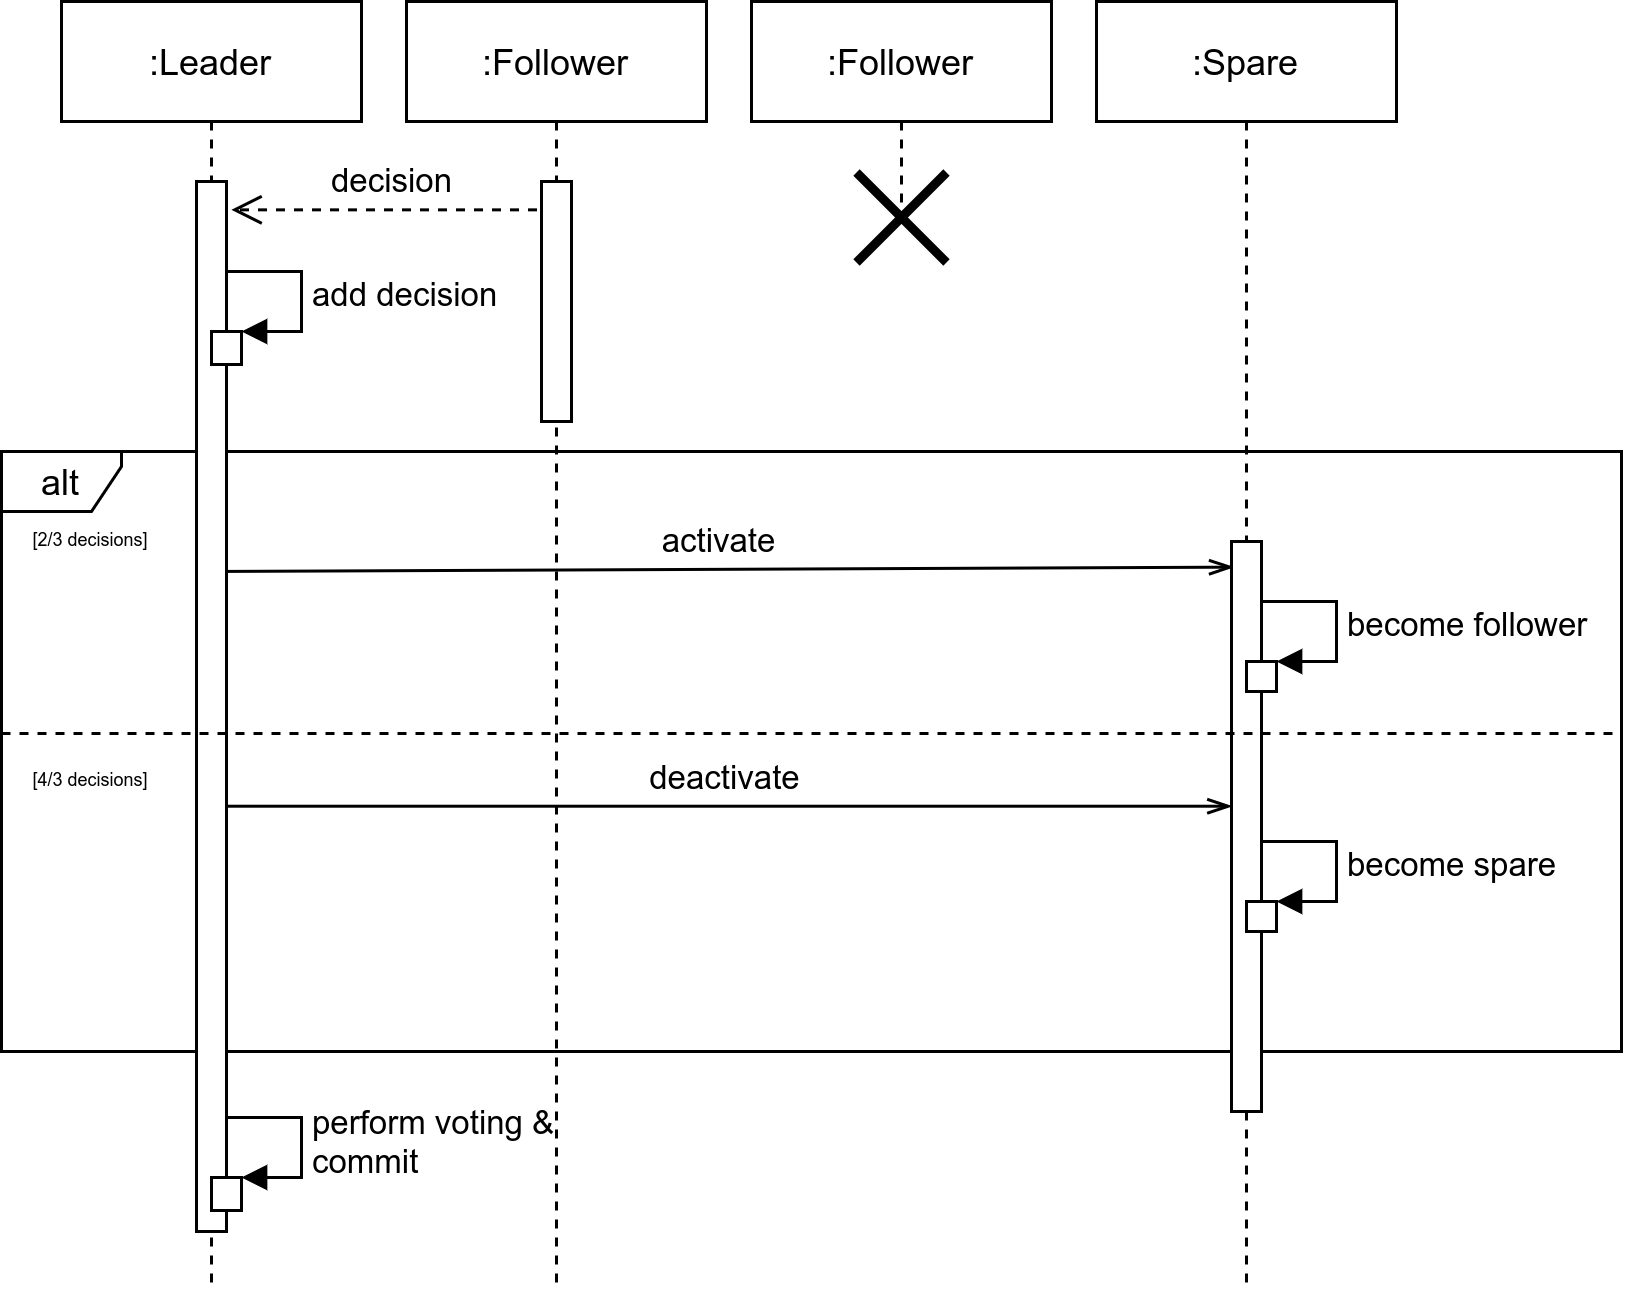
\includegraphics[width=0.75\linewidth]{images/sequence/ActivateSpare}
	\caption{When the leader, after reading an input message and instructing its followers to process the input, receives too few decisions after a certain time, it activates the spare replica. When the follower receives more than necessary, the spare component gets deactivated again.} as well as replies to vote requests
	\label{fig:SeqActivateSpare}
\end{figure}

A method for adding hot standby spare replicas to the system using \abr{DDS} topics has been depicted in~\autoref{fig:TMRWithSparesDDS}.
To put this approach into practice, a new topic was introduces, called \texttt{ActivateSpare}, whose \abr{IDL} is shown in~\autoref{code:activateSpare}.
Any activate and deactivate message is sent via the \texttt{ActivateSpare} topic.
The additional logic merges into the log replication logic and is depicted in~\autoref{fig:SeqActivateSpare}.
When collecting all decisions from the follower replicas, the leader activates or deactivates the spare component when receiving too few or too much decisions, respectively.
Any spare replica is initialized in spare mode and thereby excluded from making decisions, from becoming a candidate or leader, and from participating in the leader election process.
After being activated by the leader, the spare component transitions into follower state and can therefore make decisions when asked by the leader and vote for new leaders during the leader election process.
%However, since they are required to be deactivated when too many replicas are active, any replica that has been a spare component is excluded from becoming the system's leader.

While being in \texttt{Spare} state, a replica utilizes a \texttt{WaitSet} to wait for any activate message.
When an activated spare component receives a message from the leader that should be processed, it checks whether the leader has deactivated the spare beforehand.
When this is the case, it transitions into \texttt{Spare} mode again and discards any other message.
Because of timing issues such as network delays, it can happen that an activated spare receives a \textit{deactivate} message after it processed the leader's order.
Therefore, it can happen that the leader gets more replies than there are active components in the system.
It is the leader's responsibility to handle these additional decisions appropriately.
\\

Only a single spare component is currently supported in the exemplary implementation.
However, multiple spare components can easily be added by introducing a \texttt{spareID} field in the topic's data that encodes the identification number for the spare to activate.


% TODO Further specify
\iffalse

However, without any further treatment, only crash faults can be tolerated for voters in this setup.
Methods for detecting and handling time and omission faults exist but require additional hardware.
However, since the leader has sole control about the system's output, it is impossible to tolerate computation faults in this way.
Thus, it needs to be assured that neither a voter, nor a replica of type (B), have any omission, timing, or computation fault.



Using replicated voters with a consensus algorithm, \ChallengeVoter can be solved, because the voter is no single point of failure anymore.
\fi

